\chapter{Ergebnisse und Evaluation}
Das Ergebnis der fertigen Anwendung hat die Erwartungen erf�llt. Die Systemqualit�t wird durch eine Reihe von Verbesserung deutlich erh�rt. Um Feedback und Testen wird die Arbeit mit $36$ Videos durchgef�hrt. Die Videos haben ein Framerate von 10 Frame pro Sekunde und leisten die Aufl�sung von 1080x720. Um multiperspektivische Ergebnisse zu bekommen, wird die Testvideos in verschiedenen R�ume gedreht. Die Testvideos wurden eine nach einander getestet, deswegen ver�ndert sich die Bilder auch ganz stark. Auf diesem Grund wird eine Abwechselung des Testvideos auch als eine Drehung der Kamera betrachtet, weil das Hintergrundbild auch bei Drehung stark sich �ndert. Im Allgemein kann das Programm au�ergew�hnliche Situation einer Person genau erkennen und das erf�llt das Ziel der Arbeit. Zur Visualisierung wird ein au�ergew�hnliche Situation mit einer gekreuzten Begrenzungsbox maskiert, wo die Testperson sich stattfindet. Die alle Testvideo wurden markiert, in welchen Zeitraum ist eine au�ergew�hnliche Situation passiert. Das Programm kann alle au�ergew�hnliche Situation erkennen, wo die Testperson auf dem Boden liegt und sich nicht mehr in 15 Bilder bewegt. Bei der Markierung wurden die au�ergew�hnliche Situation genau dann notiert, wenn die Testperson anfangt, auf dem Boden zu liegen. Auf diesem Grund wird das Programm nicht 100\% schaffen die Situation in jeder Zeitraum zu erkennen. Es wird hier nur die betrachtet, ob das System die au�ergew�hnliche in einem Zeitraum richtig detektieren kann. Zum Beispiel wird eine abnormale Situation von Frame 100 bis 200 notiert und unseres System sagt von Frame 120 bis 210. Dann das ist nicht 100\% richtig, aber die Erkennung von der abnormale Situation von Frame 100 bis 200 ist erfolgreich.\\

F�r Messung der Laufzeit wurden die Tests auf einem Rechner Intel-Core i5 2.60 GHz ausgef�hrt. Die Laufzeit wird mehr mal gemessen und f�r jedes Bild braucht das System ein durchschnittlicher Wert von 109 Millisekunde die Verarbeitungszeit. Das bedeutet in eine Sekunde kann das System 100 Bilder mit Aufl�sung von 1280x720 schaffen. Damit wird auch unseres zweite Ziel realisiert und das Programm ist eine Echtzeitanwendung zur Erkennung der au�ergew�hnlichen Situation. Die Abbildung \ref{fig:laufzeit} stellt eine Laufzeit von 1000 Bilder in graphisch dar.\\


\begin{figure}[htpb]
	\centering
	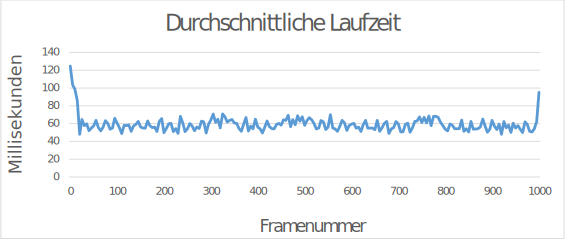
\includegraphics[width=1\textwidth]{fig/laufzeit.pdf}
	\caption{Laufzeit in 1000 Bilder} 
	\label{fig:laufzeit}
\end{figure}